\begin{answer}
    \begin{figure}[H]
        \centering
        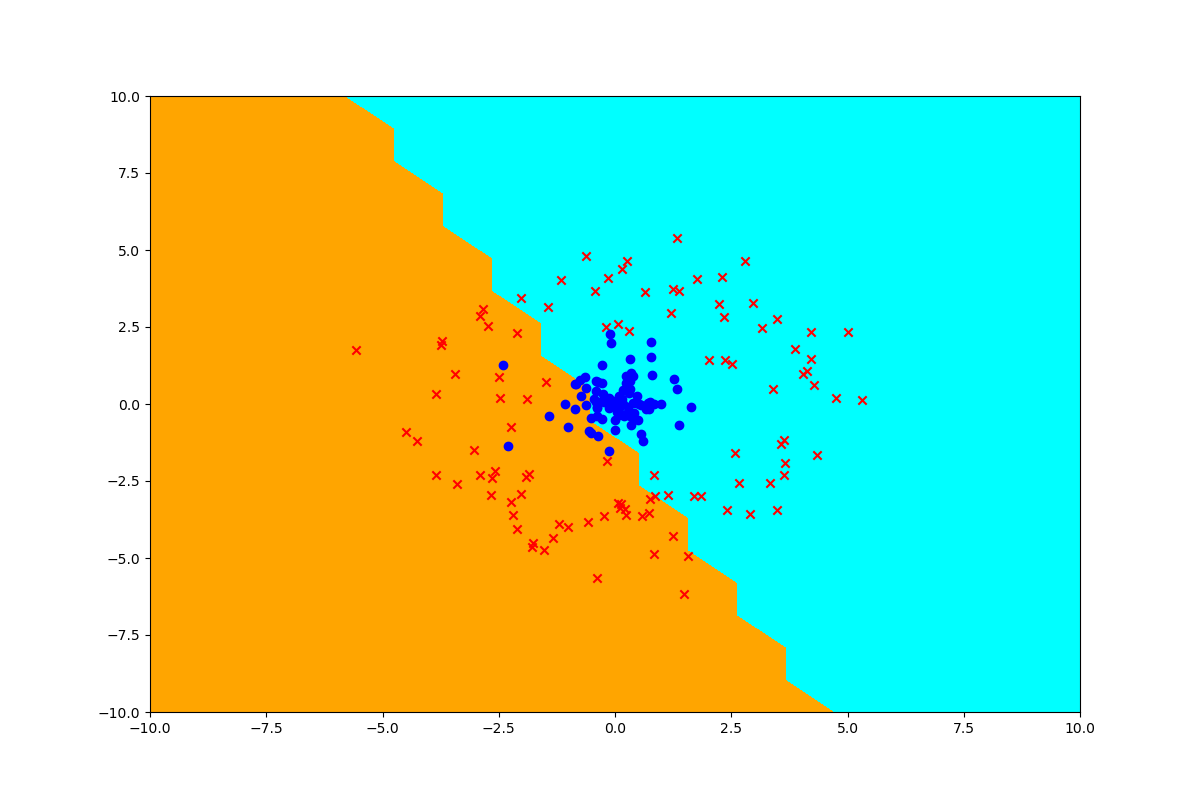
\includegraphics[width=0.75\textwidth]{../src/perceptron/perceptron_dot_output.png}
        \caption{Dot-product kernel}
        \label{fig:dot-product}
    \end{figure}
    \begin{figure}[H]
        \centering
        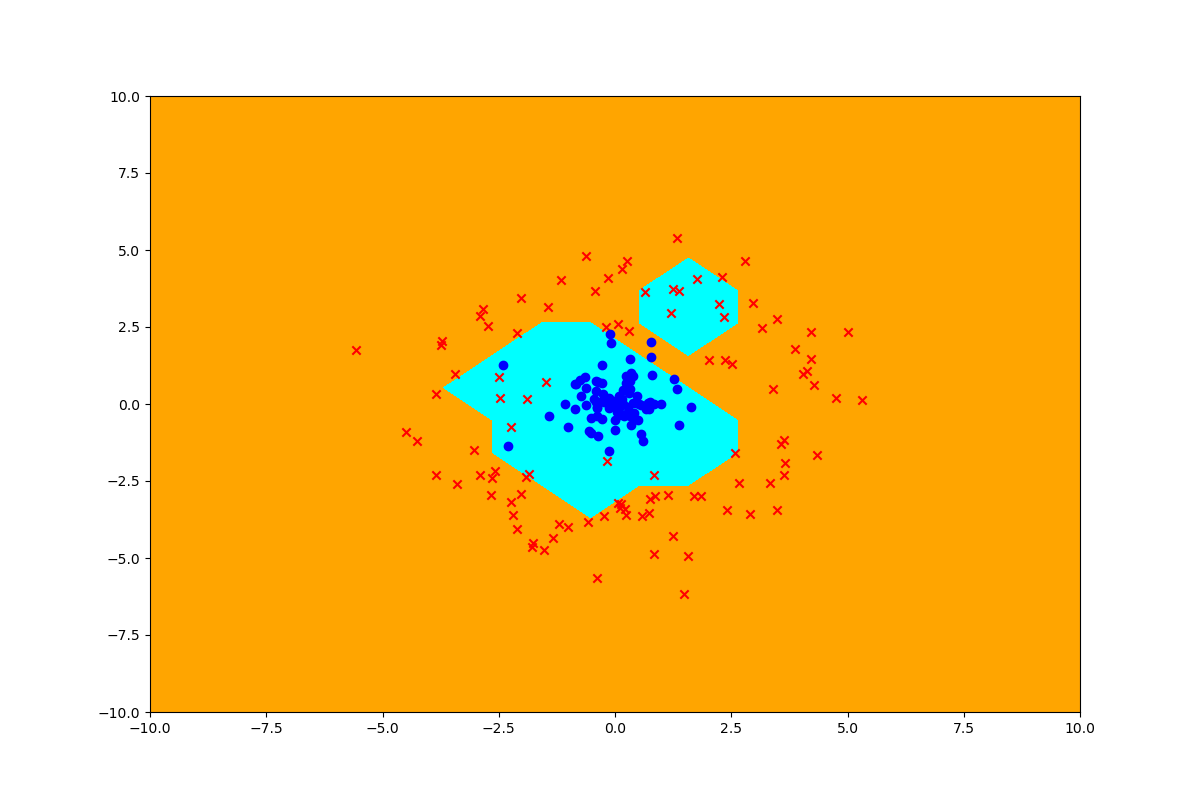
\includegraphics[width=0.75\textwidth]{../src/perceptron/perceptron_rbf_output.png}
        \caption{RBF kernel}
        \label{fig:rbf}
    \end{figure}
    \begin{figure}[H]
        \centering
        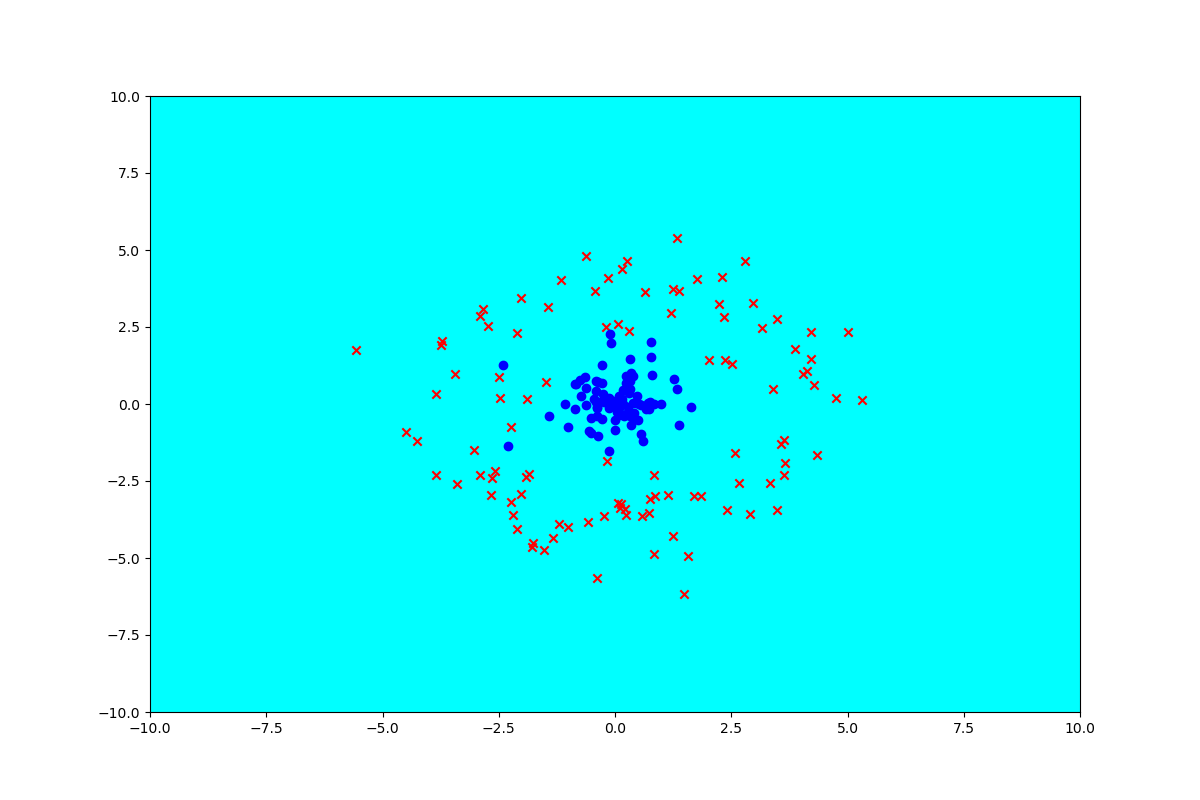
\includegraphics[width=0.75\textwidth]{../src/perceptron/perceptron_non_psd_output.png}
        \caption{Non PSD kernel}
        \label{fig:non_psd}
    \end{figure}
\end{answer}
